\section{Equations of motion}\label{sec:2.3}
I would like now to write the equations of motion of an electron that is moving on a trajectory near the design orbit, and with an energy near, but not necessarily at, the design energy. I shall describe the energy of the electron in terms of the deviation $\epsilon$ from the design energy $E_0$:
\begin{align}
	\epsilon = E-E_0
\end{align}
In keeping with our linear approximation I shall keep terms only to first order in the ``small'' quantities $x$, $y$, and $\epsilon$. Rather than using time as the independent variable it will be more convenient to use the azimuthal coordinate $s$. Derivatives with respect to $s$ will be indicated by the ``prime'' ($'$); for example, $x' = dx/ds$.

Let’s begin with the radial motion. Think of an electron that is at $x$ and moving with the slope x’. See Fig.~\ref{fig:fig9}. The slope $x'$ is the angle between the direction of motion of the electron and the tangent to the design orbit. Suppose we call $\theta_0$, the angle between the tangent and some arbitrary reference direction and $\theta$ the angle made by the trajectory with the same reference direction. Then $x' = \tan(\theta - \theta_0) \approx \theta - \theta_0$; and
\begin{align} \label{eq:2.12}
	x'' = \frac{d(\theta-\theta_0)}{ds}.
\end{align}

\begin{figure}[!htb]
	\centering
	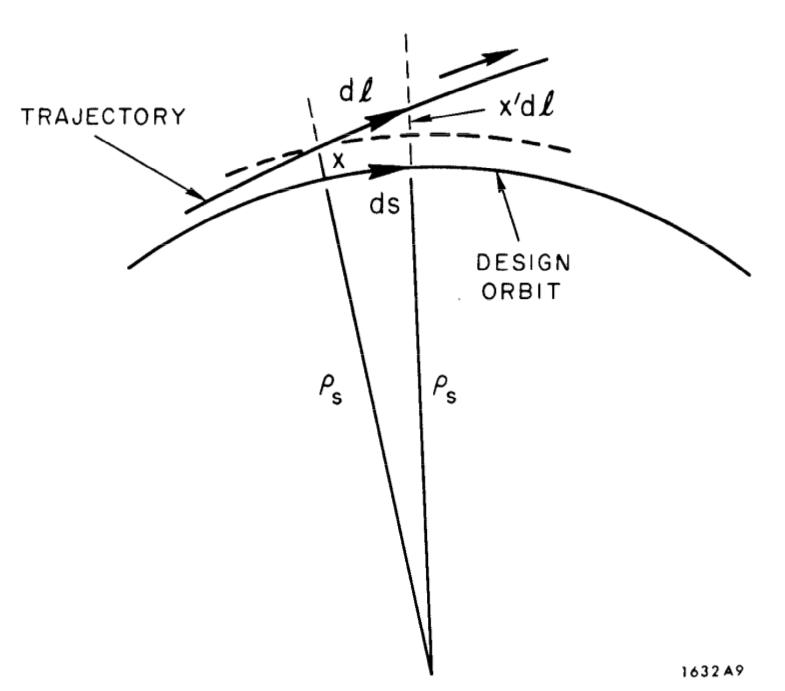
\includegraphics[width=0.6\linewidth]{./Figuras/fig09.jpeg}
	\caption{Electron trajectory near the design orbit.}
	\label{fig:fig9}
\end{figure}

The derivative of $\theta_0$ is, we have seen, just $-1/\varrho_s = -G(s)$. But what is $d\theta/ds$? The radius of curvature of the trajectory is
\begin{align} \label{eq:2.13}
	\varrho = \frac{E}{ecB},
\end{align}
and in a path element $d\ell$ of the trajectory the change in angle is
\begin{align}
	d\theta = -\frac{d\ell}{\varrho} = -\frac{ecB}{E}d\ell\label{eq:2.14}.
\end{align}

Since $\frac{d\ell}{ds} = \frac{d\ell}{d\theta}\frac{d\theta}{d\theta_0}\frac{d\theta_0}{ds}$, then

\begin{align*}
\frac{d\ell}{ds} = \left(-\varrho\right)\frac{d\theta}{d\theta_0}\left(-\frac{1}{\varrho_s}\right).
\end{align*}

Next, notice that so long as the angle $x'$ is small -- as I shall always assume -- the variations of angles $\theta$ and $\theta_0$ are approximately the same in first order,
so $\frac{d\theta}{d\theta_0} \approx 1$. Moreover, the radius of curvature $\varrho$ is $\varrho \approx \varrho_s + x$ in first order again. Thus, a path element $d\ell$ of a trajectory at
$x$ is related to the corresponding change in $s$ by

\begin{align}
	d\ell = \frac{\varrho_s + x}{\varrho_s} ds = \left(1+\frac{x}{\varrho_s}\right)ds = (1+G(s)x)ds\label{eq:2.15}
\end{align}
Next, we may write for $B$
\begin{align}
	B = B_0 + \frac{\partial B}{\partial x}x = \frac{E_0}{ec}(G+K_1x)\label{eq:2.16}
\end{align}
Putting these two into \eqref{eq:2.14} -- together with $E_0 + \epsilon$ for $E$ -- and keeping only first order terms, we find that
\begin{align*}
	d\theta = \left\{-G-(G^2+K_1)x + G\delta\right\}ds
\end{align*}
And so we get from \eqref{eq:2.12} that
\begin{align}\label{eq:2.17}
	x'' = -(G^ 2+K_1)x + G\delta
\end{align}

\begin{proof}
	From \eqref{eq:2.14},
	\begin{align*}
		d\theta &= -\frac{ecB}{E}d\ell\\
				&= -\frac{ecB}{E}(1+Gx)ds\\
				&= -\frac{ec}{E}\left[\frac{E_0}{ec}(G+K_1x)\right](1+Gx)ds\\
				&= -\frac{E_0}{E_0+\epsilon}(G+K_1x)(1+Gx)ds\\
				&= -\frac{E_0}{E_0+\epsilon}(G+(G^2+K_1)x + K_1Gx^2)ds
	\end{align*}

    Keeping only terms to first order,
	\begin{align*}
		d\theta &= \frac{1}{1+\delta}(-G-(G^2+K_1)x)ds
	\end{align*}

	$\delta$ is very small, so we can consider that $\frac{1}{1+\delta}$ is just  the sum of a geometric series. So, we can expand this term in a summatory:
	\begin{align*}
		d\theta &= \left(1 - \delta + \delta^2+ ...\right)(-G-(G^2+K_1)x)ds
	\end{align*}

    Again, keeping only terms to first order,
	\begin{align*}
		d\theta &= \left(1 - \delta\right)(-G-(G^2+K_1)x)ds\\
				&= (-G-(G^2+K_1)x)ds + \left(G\left(\delta\right)+(G^2+K_1)x\left(\delta\right)\right)ds\\
				&= \left\{-G-(G^2+K_1)x + G\delta\right\}ds
	\end{align*}

	Now, from \eqref{eq:2.12},
	\begin{align*}
		x'' &= \frac{d(\theta-\theta_0)}{ds}\\
			&= \left\{-G-(G^2+K_1)x + G\delta\right\} - (-G)\\
			&= -(G^2+K_1)x + G\delta
	\end{align*}
\end{proof}

The corresponding equation for the vertical motion is easier to derive; you can easily see that
\begin{align}
	y'' = K_1 y
\end{align}

\begin{proof}
	For the vertical motion, applying the Lorentz force, we can see that it has the opposite sign from the radial motion:

	\begin{align*}
		d\theta &= -\frac{d\ell}{\varrho} = + \frac{ecB}{E}d\ell =  K_1 y ds.
	\end{align*}

 We have used the fact that there is no horizontal dipole component, therefore for the vertical plane the field expansion has only a linear term $\frac{ecB}{E} = K_1 y$ and $d\ell = ds$.

	Now, from \eqref{eq:2.12},
	\begin{align*}
		y'' &= \frac{d(\theta-\theta_0)}{ds}\\
			&= \frac{K_1 y\ ds}{ds}\\
			&= K_1 y
	\end{align*}
	keeping in mind that $\frac{d\theta_0}{ds} = 0$ comes from the assumption that the design orbit lies in a horizontal plane.
\end{proof}

Notice that with our linearized approximation, the motions in $x$ and $y$ are independent. For our consideration of the electron trajectories, I would like to use the standard form:
\begin{align}
	x'' &= -K_x(s)x + G(s)\delta\label{eq:2.19}\\
	y'' &= -K_y(s)y\label{eq:2.20}
\end{align}
with the definitions:
\begin{align}
	K_x(s) &= G^2(s)+K_1(s) \label{eq:2.21}\\
	K_y(s) &= -K_1(s) \label{eq:2.22}
\end{align}
The term corresponding to $G^2$ is missing from $K_y$ because of our assumption that
the design orbit lies in a plane. Storage rings are most often ``strong focusing''. For such rings $G^2$ is generally much smaller than $K_1$, so that $K_x$ and $K_y$ are approximately equal and have opposite signs.

The equation for the motion in $y$ looks like the equation of a classical oscillator (force proportional to displacement) with a variable ``restoring-force'' coefficient -- the function $K_y(s)$. The equation in $x$ is similar except that it has, in addition, a varying ``driving term'' which is proportional to the energy deviation $\epsilon$. In useful guide fields the solutions are indeed oscillatory, and describe the \textit{lateral oscillations} -- including the so-called \textit{betatron} oscillations -- of the electron trajectories. These oscillations result from the \textit{focusing} properties of the guide field which are characterized by \textit{focusing functions} $K_x$ and $K_y$. As we shall see later, the function $G(s)$ enters as well in the \textit{energy focusing} properties of the guide field.

It is important to remember that all of the focusing functions are necessarily periodic in $s$, the minimum period being one revolution of the ideal orbit; that is, for both $K_x$ and $K_y$ (as well as for $G$)
\begin{align}
	K(s+L) = K(s)\label{eq:2.23}
\end{align}
where $L$ is the length of the ideal orbit. For convenience in construction -- as well as in design -- storage rings generally have also an inner periodicity. That is, they are made up,at least in part, of sequences of identical magnetic \textit{cells},
each cell consisting of a prescribed set of magnets and quadrupoles. Then in a certain span of $s$, the focussing functions will satisfy
\begin{align}
	\left\{\begin{array}{rcl}
	\ G(s+\ell_c) & = & G(s)\\
	K(s+\ell_c) & = & K_1(s)
	\end{array}\right.
\end{align}
where $\ell_c$ is the cell length. Note, however, that while Eq. \eqref{eq:2.23} is true for the \textit{actual} fields of a ring -- since when $s$ is increased by $L$, the electron returns to the same physical point in the ring -- the cell periodicity is a \textit{design} property and will not be strictly true for the actual fields (due to construction imperfections).

It will be useful to have in mind some illustrative example of a guide field. Let’s take the design of the proposed SLAC ring. In it, most of the ring would consist of a repetition of a standard cell, each of which occupies about 1/16 of a full circle. I show in Fig.~\ref{fig:fig10}, the nature of the focusing functions over a part

\begin{figure}[!htb]
	\centering
	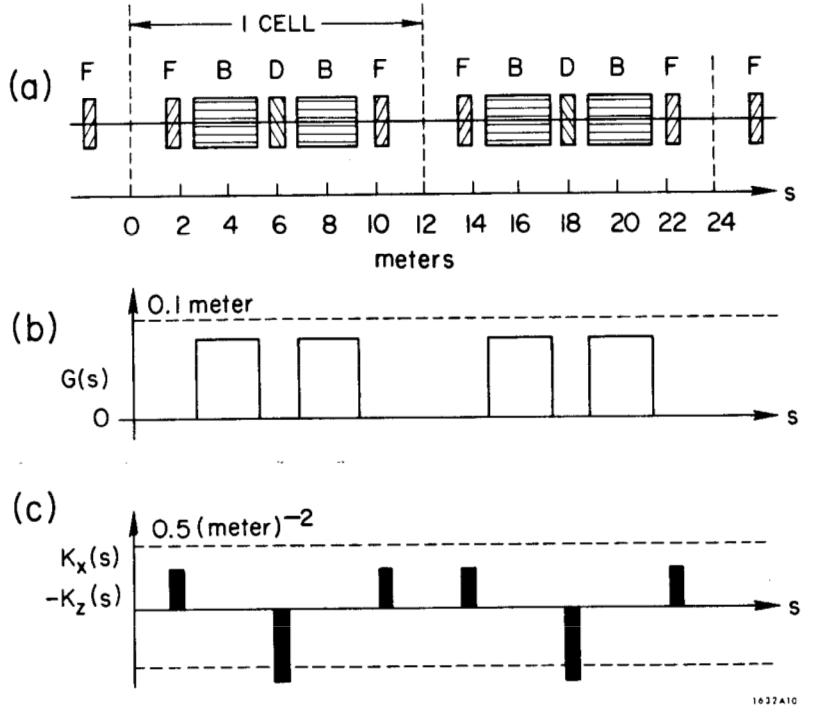
\includegraphics[width=0.7\linewidth]{./Figuras/fig10.jpeg}
	\caption{Magnet lattice and focusing functions in the normal cells
	of a particular guide field.}
	\label{fig:fig10}
\end{figure}
of the ring, comprising two such cells. Part (a) of the figure shows the layout of bending magnets and quadrupoles. The bending magnets designated B, have a uniform field $(dB/dx = 0)$; the quadrupoles have no field on the design orbit $(B_0=0)$ and are designated F or D (for focusing or defocusing in the radial motion) depending on whether their gradients are positive or negative. The other parts of the figure give the focusing functions $G$, $K_x$, and $K_y$.
